\section{Modelo de Banco de Dados} % ### 5.4. Modelo de Banco de Dados

Considerando as informações necessárias para o presente trabalho, e também o preparo de campo para potenciais aplicações futuras, foi elaborado um diagrama conceitual de banco de dados, que pode ser visto na Figura \ref{fig:DiagramConceitual}.

\begin{figure}[htbp]\centering
  \caption{\label{fig:DiagramConceitual} Diagrama Conceitual do banco de dados}
  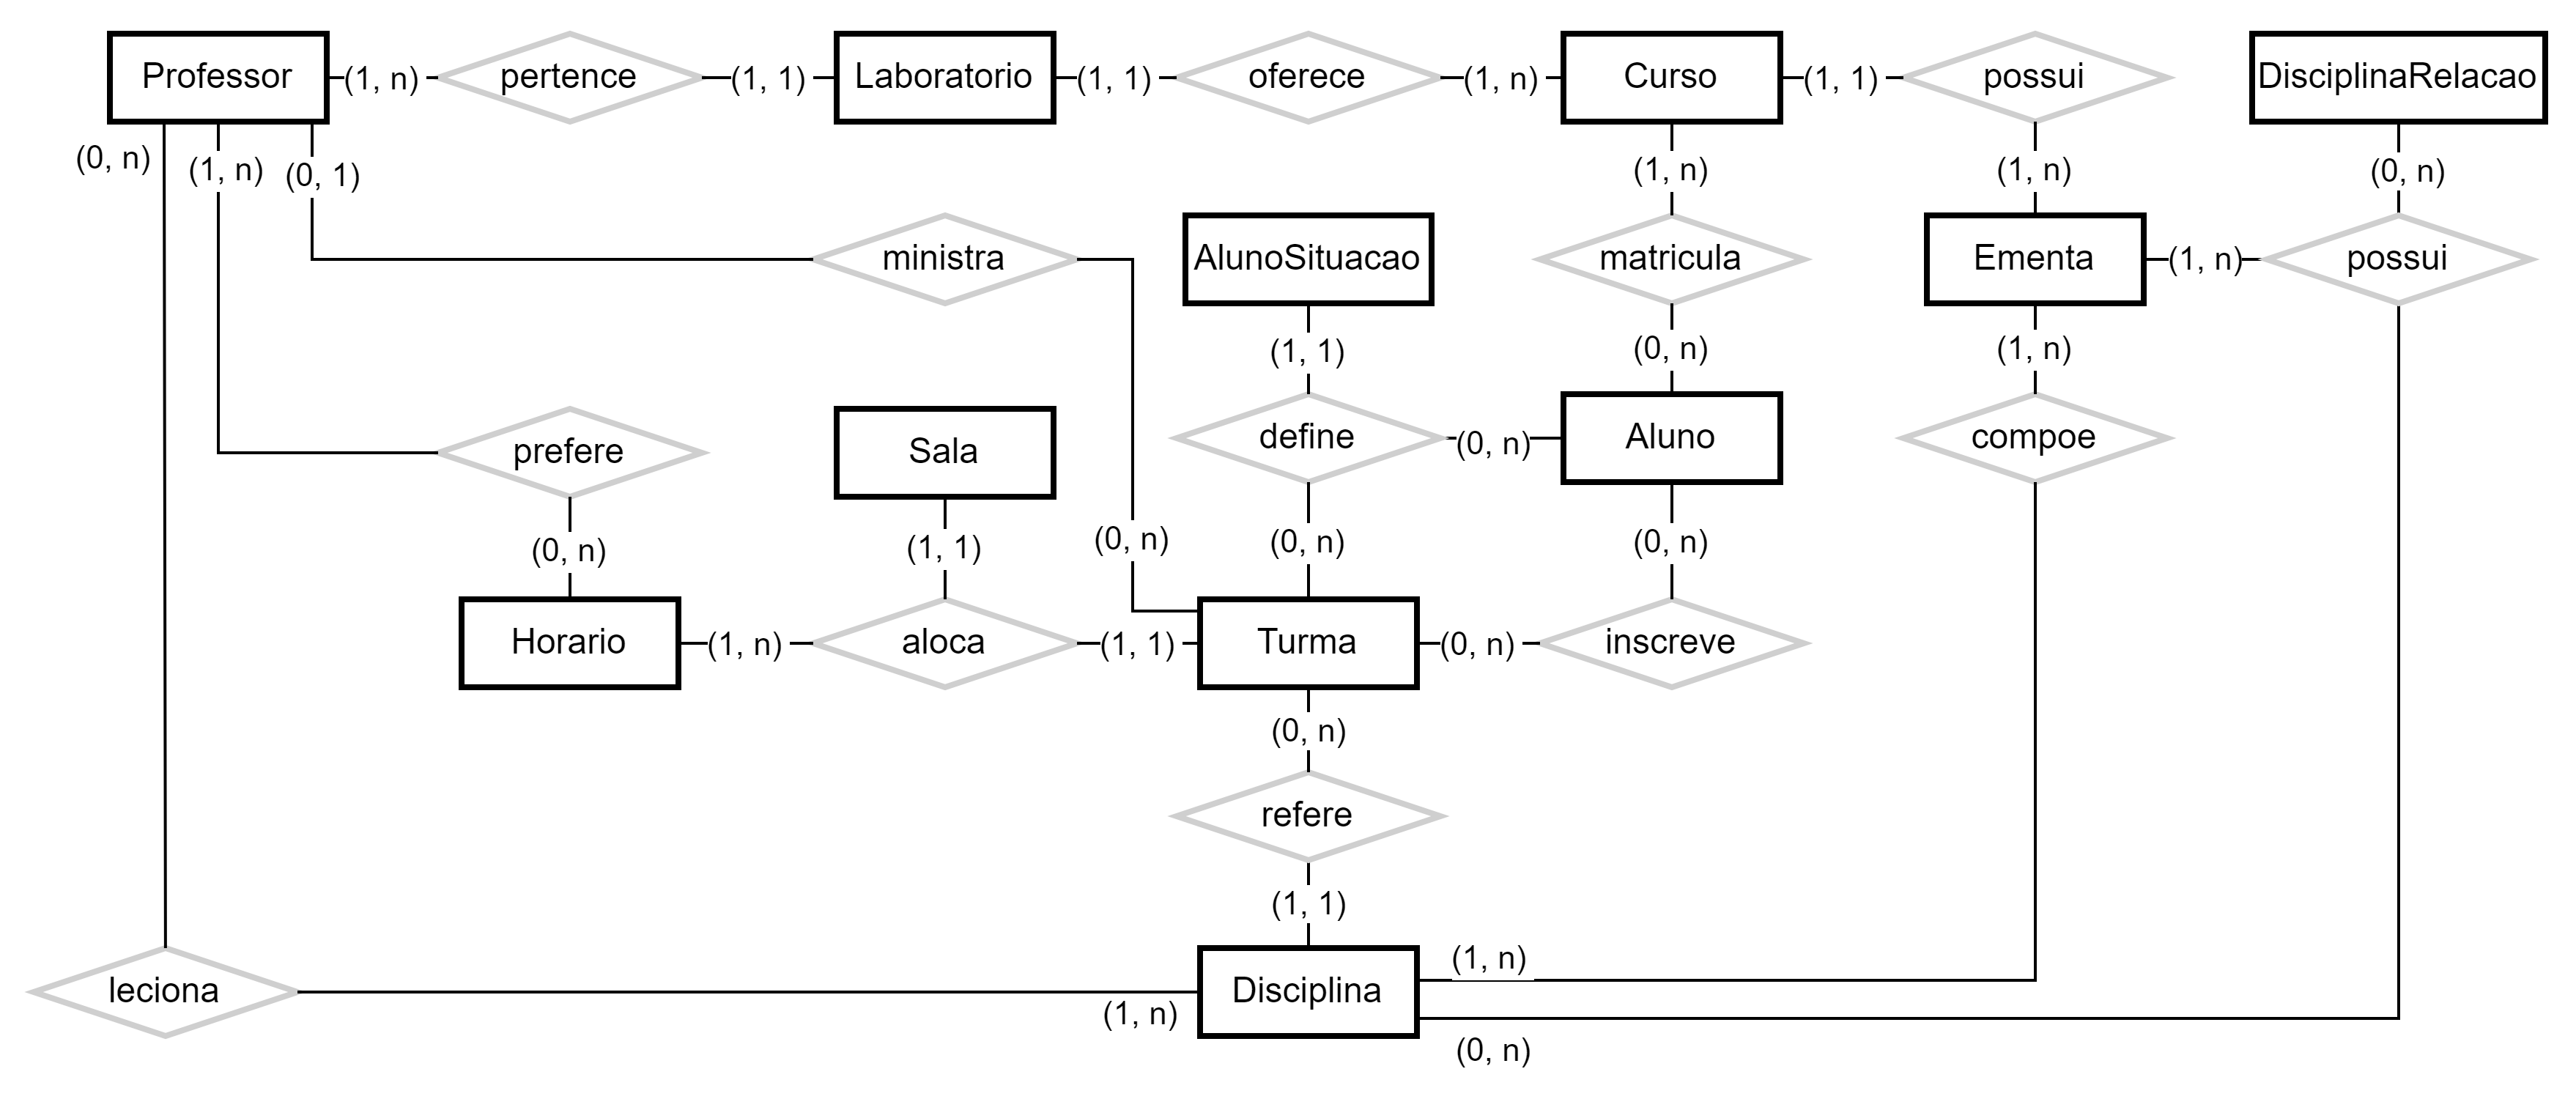
\includegraphics[scale=0.2]{files/img/DiagramaConceitual/DiagramaConceitualBranco.png}
  \legend{Fonte: o autor}
\end{figure} % Diagrama Conceitual

O diagrama conceitual foi elaborado utilizando a ferramenta \href{https://www.drawio.com/}{draw.io} citada na metodologia e ilustra as relações entre diversas entidades presentes na realidade da UENF. O emaranhamento presente no diagrama ilustra a complexidade envolvida na criação de uma grade horária, onde diversas entidades se relacionam entre si.

Como principais apontamentos, podemos citar a parte principal do modelo que é a alocação de turmas. Ela, como já descrito, envolve a correlação entre alunos de diferentes cursos, professores, disciplinas, salas e horários. Além disso, também é possível notar a presença de entidades que não são diretamente relacionadas à alocação de turmas, mas que podem se mostrar úteis, como a relação entre professores e laboratórios, e a de disciplinas e ementas.

Embora o diagrama apresente uma visão mais completa de todas as interconexões possíveis, é importante ressaltar que o presente trabalho foca primordialmente na alocação das turmas para o curso de Ciência da Computação, e que a implementação do banco de dados será feita de forma a atender a essas necessidades, fazendo então uso de uma parte do diagrama conceitual.

% Tendo isso em vista, o modelo conceitual reduzido para o presente trabalho pode ser visto na Figura \ref{fig:DiagramConceitualReduzido}.

% \begin{figure}[htbp]\centering
%   \caption{\label{fig:DiagramConceitualReduzido} Diagrama Conceitual reduzido para o presente trabalho}
%   \includegraphics[scale=0.2]{files/img/DiagramaConceitual/DiagramaConceitualReduzidoBranco.png}
%   \legend{Fonte: o autor}
% \end{figure} % Diagrama Conceitual reduzido

Neste modelo, mais enxuto, temos apenas as entidades principais, onde temos uma turma de determinada disciplina, ministrada por um professor e que ocorre em uma sala em um determinado horário.

